\chapter{Solution Application}
\label{ch:SolutionApplication}
This chapter applies the previously presented approach to identify microservices from the business point of view, using clustering on control flow and data flow. It is applied to the case study CoCoME, whose system specifications are defined in chapter \ref{ch:CoCoME}. Speaking of the order, this chapter follows the process overview illustrated by Fig.\ref{fig:thesisProcess}.

\section{Specify BPMN Models}
CoCoME's system specifications are given in terms of use cases. A short overview is available in chapter \ref{ch:CoCoME}, whereas a more detailed version can be found in the \textit{Technical Report} \cite{CoCoMETechnical}. We decide to omit  \textit{UC 8 - Product Exchange} as independent BPMN model, because both reference sets either did not take it into consideration or implemented it differently. However, it was added as extension to \textit{UC 1} as single activity named \textit{Product Exchange}. In the same way, \textit{UC 2 - Manage Express Checkout} is added to \textit{UC 1} as single activity named \textit{Manage Express Checkout}. \textit{UC 2} extends \textit{UC 1} and therefore, has to be associated with \textit{UC 1} anyway.  Fig.\ref{fig:UC1} illustrates \textit{UC 1,2} and \textit{8} as BPMN model. The remaining BPMN models are available in the appendix (cf. \ref{sec:appendix:BPMN Models}). For the sake of clarity, the models are not yet joined as described in section \ref{sec:PrepApproach:TransformUCtoBPMN}. Apart from Fig.\ref{fig:UC1}, each use case is illustrated as single BPMN process. However, the BPMN models that represent \textit{UC 3} and \textit{UC 4} as well as \textit{UC 4} and \textit{UC 1} need to be joined, as preconditions and postconditions are equal. 

%TODO Connection 


%"l, b, r, t"
\begin{figure}[h!]
	\centering
	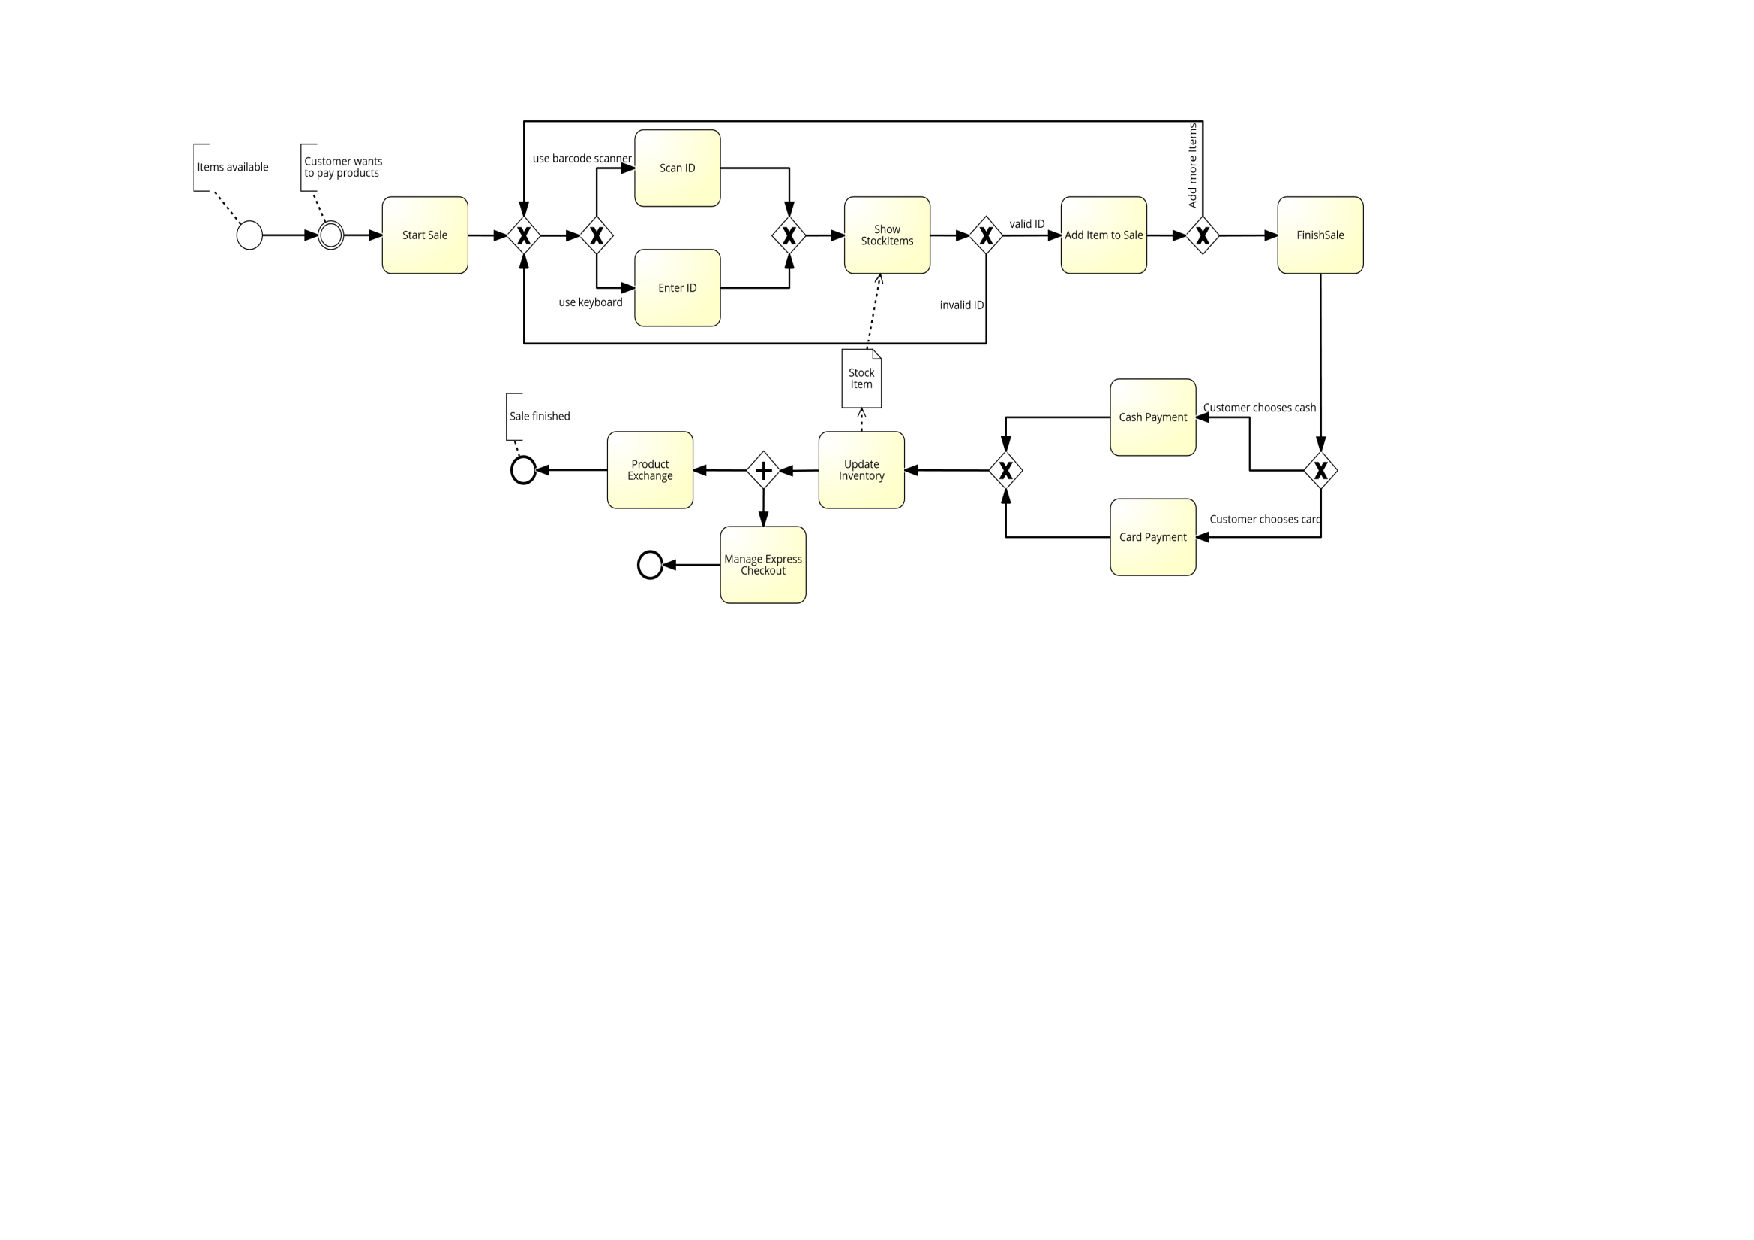
\includegraphics[width=\textwidth, trim={4cm 10.5cm 8cm 2cm}]{img/UC1.pdf}
	\caption{UC1-Process Sale (with UC2 and UC8)}
	\label{fig:UC1}
\end{figure}




\section{Extract Control Flow}

Connection

\section{Extract Data Flow}

\section{Create weighted Graphs using Control Flow}

\section{Create weighted Graph using Data Flow}

\section{Identify Clusters}

\section{Match Clusters}

\section{Extract Microservice Candidates}